\section{Empirical Results}\label{sec:results}

\section{Data}\label{subsec:data}
In the empirical analysis, we consider the risk reduction capability of the BTC-future (BTCF) on five cryptos
, BTC, ETH, ADA, LTC, and XRP, and five crypto indexes, BITX, BITW100, CRIX, BITW20, and BITW70,
For each of the 10 hedging portfolios, a crypto or index is considered as the spot and held in a unit size long position,
and the BTCF is held in short position of OHR unit in order to reduce the risk of the spot.
All the hedging portfolios are cross asset hedging except the BTCF portfolio.
ETH, ADA, LTC, and XRP are popular cryptos tradable in various exchanges and have large market capitalization.
BITX, BITW100, and CRIX are market-cap weighted crypto indexes with BTC as constituent.
BITX and BITW100 tracks the total return of the 10 and 100 cryptos with largest market-cap respectively.
CRIX decides the number of constituents by AIC and track that number of cryptos with largest market-cap.
In our case, the number of constituents in CRIX is 5.
BITW20 is also a market-cap weighted crypto index but with 20 largest market-cap cryptos outside the constituents of
BITX.
BITW70 has the same construction as BITW20 but with 70 largest market-cap cryptos outside BITX and BITW20.
Therefore, BTC is excluded as constituent in BITW20 and BITW70. \medskip

We collect the spots' and BTCF's daily price at 15:00 US Central Time (CT).
The reason of choosing this particular time is that the CME group determines the daily settlements for BTCFs based on the trading activities on CME Globex between 14:59 and 15:00 CT.
15:00 CT is also the reporting time of the daily closing price by the Bloomberg Terminal (BBT).
Cryptos data are collected from a data provider called Tiingo.
Tiingo aggregates crypto OHLC (open, high, low, and close) prices fed by APIs from various exhcanges.
Tiingo covers major exchanges, e.g. Binance, Gemini, Poloniex etc., so Tiingo's aggregated OHLC price is a good representation a market tradable price.
For each crypto, we match the opening price at 15:00 CT from Tiingo with the daily closing price of BTCF from BBT.
Since CRIX is not available at 15:00 CT, we recalculate a hourly CRIX using the monthly constituents weights and the hourly OHLC price data collected from Tiingo.
BITX, BITW20, BITW70, and BITW100 are collected from the official website of their publisher Bitwise.com.
The daily reporting time of the Bitwise indexes is 15:00 CT. \medskip

At the time of writing, the CRIX' is undergoing the listing process on the S\&P Dow Jones Indices,
the official CRIX data will then be calculated with Lukka Prime Data and available to public via S\&P.



















%\francis{\em This section is under construction}
%Cryptocurrenices are traded around the clock, but CME future are traded from
%Sunday to Friday from 05:00 p.m. to 04:00 p.m. U.S. central time.
%We match the timestamps and timezones of different data sources.
%
%
%\begin{table}[htbp]
%    \centering
%    \begin{tabularx}{\textwidth}{s|CCCCCCCC}
%      \hline\hline
%     \# & Asset & Data Source & Type & Tradable at CT\footnotemark & Tradable at CET\footnotemark during CST\footnotemark & Tradable at CET during CDT\footnotemark & Tradable at UTC during CST & Tradable at UTC during CDT\\       \hline
%      1 & Bitcoin & Coingecko API & Hourly Close &  & 11:00pm D+0 & 11:00pm D+0 & 10:00pm D+0$^*$ &10:00pm D+0$^*$ \\\hline
%      2 & CME Future & Bloomberg & Daily Open & 05:00pm D-1 & 00:00am D+0$^*$ & 00:00am D+0$^*$ & 11:00pm D-1 & 10:00pm D-1 \\       \hline
%      3 & CME Future & Bloomberg & Daily Close & 04:00pm D+0& 11:00pm D+0$^*$ & 11:00pm D+0$^*$ & 10:00pm D+0 & 09:00pm D+0\\       \hline
%      4 & CRIX & IRTG (from Coingecko) & Index &  &  &  & & 00:00am D+0$^*$\\\hline
%    \end{tabularx}
%    \caption{$^*$ indicates the timestamp of raw data from data source. }
%    \label{tab:table}
%\end{table}
%
%\addtocounter{footnote}{-3}
%\footnotetext{CT stands for U.S. Central Time. It represents two observances of time, the Central Standard Time (CST) and the Central Daylight Time (CDT)}
%\addtocounter{footnote}{1}
%\footnotetext{CET stands for Central European Time. It is one hour ahead UTC.}
%\addtocounter{footnote}{1}
%\footnotetext{CST is six hours behind UTC.}
%\addtocounter{footnote}{1}
%\footnotetext{CDT is five hours behind UTC.}
%
%Hedging Pair 1 is hedging \#1 (Bitcoin Spot) with \#3 (CME future).
%The time difference between the two prices is zero.
%They are both adjusted to CET time:
%\#1 by pandas.Series.dt.tz\_convert; \#3 by retrieving data from Bloomberg Terminal located in Berlin. \medskip
%
%Hedging Pair 2 is hedging \#4 (CRIX) with \#2 (CME future).
%We observe \#2 two hours and one hour before \#4 during CST and CDT respectively.
%
%
%\subsection{Time Difference}\label{subsec:time-difference}
%\begin{table}[h]
%    \centering
%
%\begin{tabular}{lrrrr}
%\toprule
%{} &     Open &     High &      Low &    Close \\
%\midrule
%2021-02-02 23:00 &  36360.0 &  38155.0 &  36240.0 &  37790.0 \\
%2021-02-01 23:00 &  34205.0 &  36665.0 &  34070.0 &  36535.0 \\
%2021-01-31 23:00 &  33715.0 &  35280.0 &  32800.0 &  34265.0 \\
%2021-01-28 23:00 &  33995.0 &  39530.0 &  32590.0 &  35180.0 \\
%2021-01-27 23:00 &  31005.0 &  33710.0 &  30350.0 &  33085.0 \\
%\bottomrule
%\end{tabular}
%       \caption{CME Bitcoin Future Raw Data}
%    \label{tab:table0} \medskip
%
%    \begin{tabular}[width=\textwidth]{llrrrr}
%\toprule
% &                      date &           CRIX &   future &  log return CRIX &  log return future \\
%\midrule
%0 & 2021-02-04  &  104518.468839 &  38080.0 &         0.054757 &           0.046220 \\
%1 & 2021-02-03  &   98949.179255 &  36360.0 &         0.059741 &           0.061097 \\
%2 & 2021-02-02  &   93210.948461 &  34205.0 &         0.002204 &           0.014429 \\
%3 & 2021-02-01  &   93005.711051 &  33715.0 &         0.013628 &          -0.008271 \\
%4 & 2021-01-29  &   91746.863103 &  33995.0 &         0.081917 &           0.092065 \\
%\bottomrule
%    \end{tabular}
%    \caption{CRIX \#4 with Opening price of CME Bitcoin future \#2 and their log returns}
%    \label{tab:table2} \medskip
%
%\begin{tabular}{llrrrr}
%\toprule
%{} &                      date &           CRIX &   future &  log return CRIX &  log return future \\
%\midrule
%0 & 2021-02-05  &  103348.488555 &  38220.0 &        -0.011257 &           0.011314 \\
%1 & 2021-02-04  &  104518.468839 &  37790.0 &         0.054757 &           0.033774 \\
%2 & 2021-02-03  &   98949.179255 &  36535.0 &         0.059741 &           0.064146 \\
%3 & 2021-02-02  &   93210.948461 &  34265.0 &        -0.016175 &          -0.026353 \\
%4 & 2021-01-30  &   94730.919657 &  35180.0 &         0.032007 &           0.061398 \\
%\bottomrule
%\end{tabular}
%    \caption{CRIX \#4 with Closing price of CME Bitcoin future \#3 shifted for one day (D-1) and their log returns}
%    \label{tab:table3}
%\end{table}
%
%\clearpage
%\begin{figure}[ht]
%    \centering
%    \includegraphics[scale=.35]{_pics_notes/CRIX_future_Open_Close.pdf}
%    \end{figure}
%
%Kendall's tau between CRIX and future Close is 0.608429;\\
%Kendall's tau between CRIX and future Open is 0.673266; we pick this unless we have hourly CRIX.
%
%\subsection{Statistics of Percentage Difference Between CME Bitcoin future Open Price and Last Close Price}
%
%$$\text{diff} = \frac{\text{Open}_{t} - \text{Close}_{t-1}} {\text{Close}_{t-1}}$$
%
%Mean of diff = 0.00236\\
%Std of diff = 0.02206\\
%Max of diff = 0.16394 \\
%UQ of diff = 0.00814 \\
%Median of diff = 0.00132\\
%LQ of diff = -0.00412 \\
%Min of diff = -0.12190 \\


\subsection{An overview of the hedged portfolios without the copula selection step}\label{subsec:HP1}
Since different copulae may suggest different OHRs, we analyse the result of hedged portfolios without the copula selection step
in order to get a better understanding of how a copula affect the hedged portfolio with various risk minimization objectives.
To do so, we inspect the performance of copula in hedging by the mean square error and lowersemi variance.
Mean square error is the distance between a perfect hedge and the hedged portfolio returns $\operatorname{MSE}=\frac{1}{n}\sum_{i=1}^n(r^h_i)^2$.
Lower semi variance is $\operatorname{LSV}=\frac{1}{n}\sum_{i=1}^n\{\operatorname{E}(r^h)-r^h_i\}^2$.
All results here are out-of-sample results obtained without the copula selection step in order to compare the performances across copulae.  \medskip

\begin{figure}[th]
    \centering
    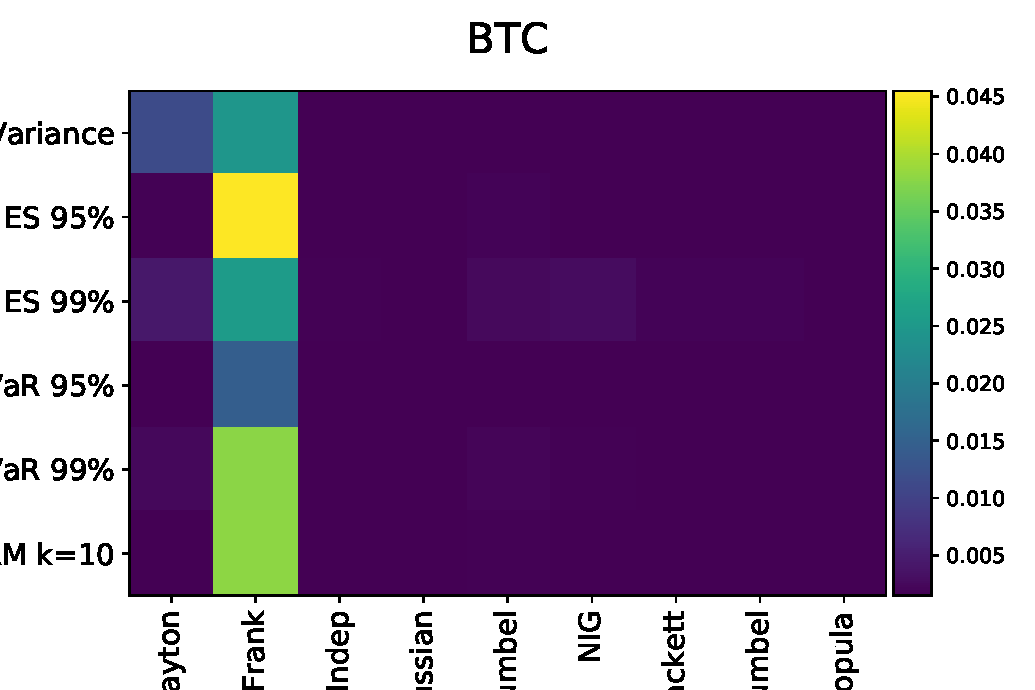
\includegraphics[width=\textwidth]{_pics/MSE_BTC.pdf}
  \caption{Mean square errors of BTC-BTCF portfolios constructed with different copula and risk minimization objectives.
    The Frank copula is inferior in the BTC-involved portfolios.
    \href{http://www.quantlet.com/}{\includegraphics[height=\baselineskip]{_pics/qletlogo_tr.png}} }
\label{fig:MSE_BTC}
\end{figure}

\begin{figure}[th]
    \centering
    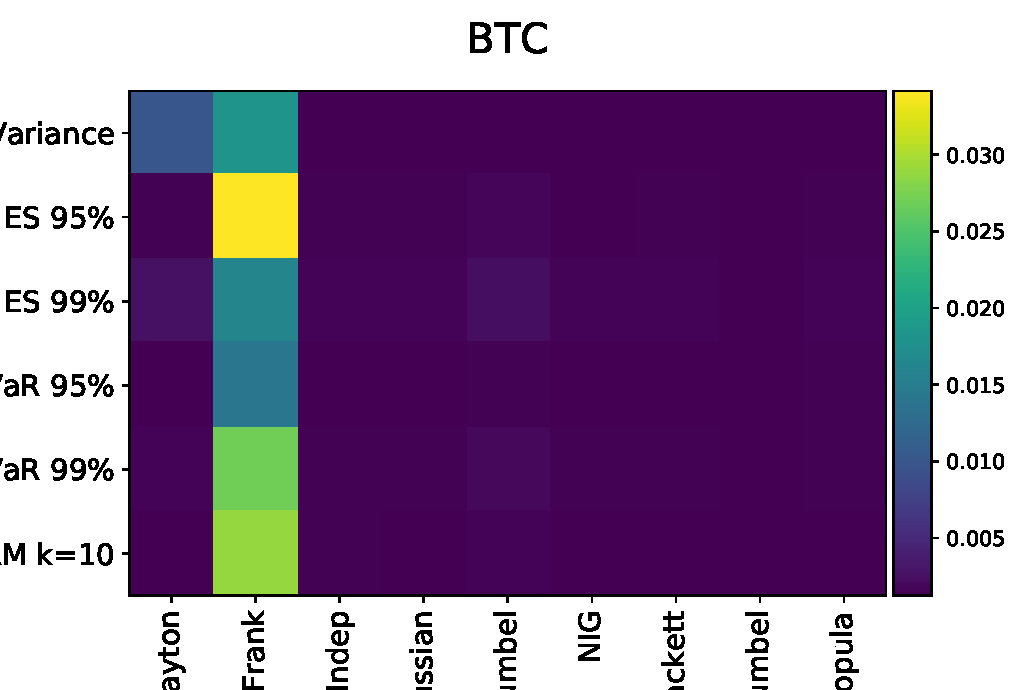
\includegraphics[width=\textwidth]{_pics/semiLowerVariance_BTC.pdf}
  \caption{Lower semivariance of BTC-BTCF portfolios constructed with different copula and risk minimization objectives.
  The Frank copula is obviously inferior.
  \href{http://www.quantlet.com/}{\includegraphics[height=\baselineskip]{_pics/qletlogo_tr.png}} }
\label{fig:SLV_BTC}
\end{figure}

\begin{figure}[th]
    \centering
    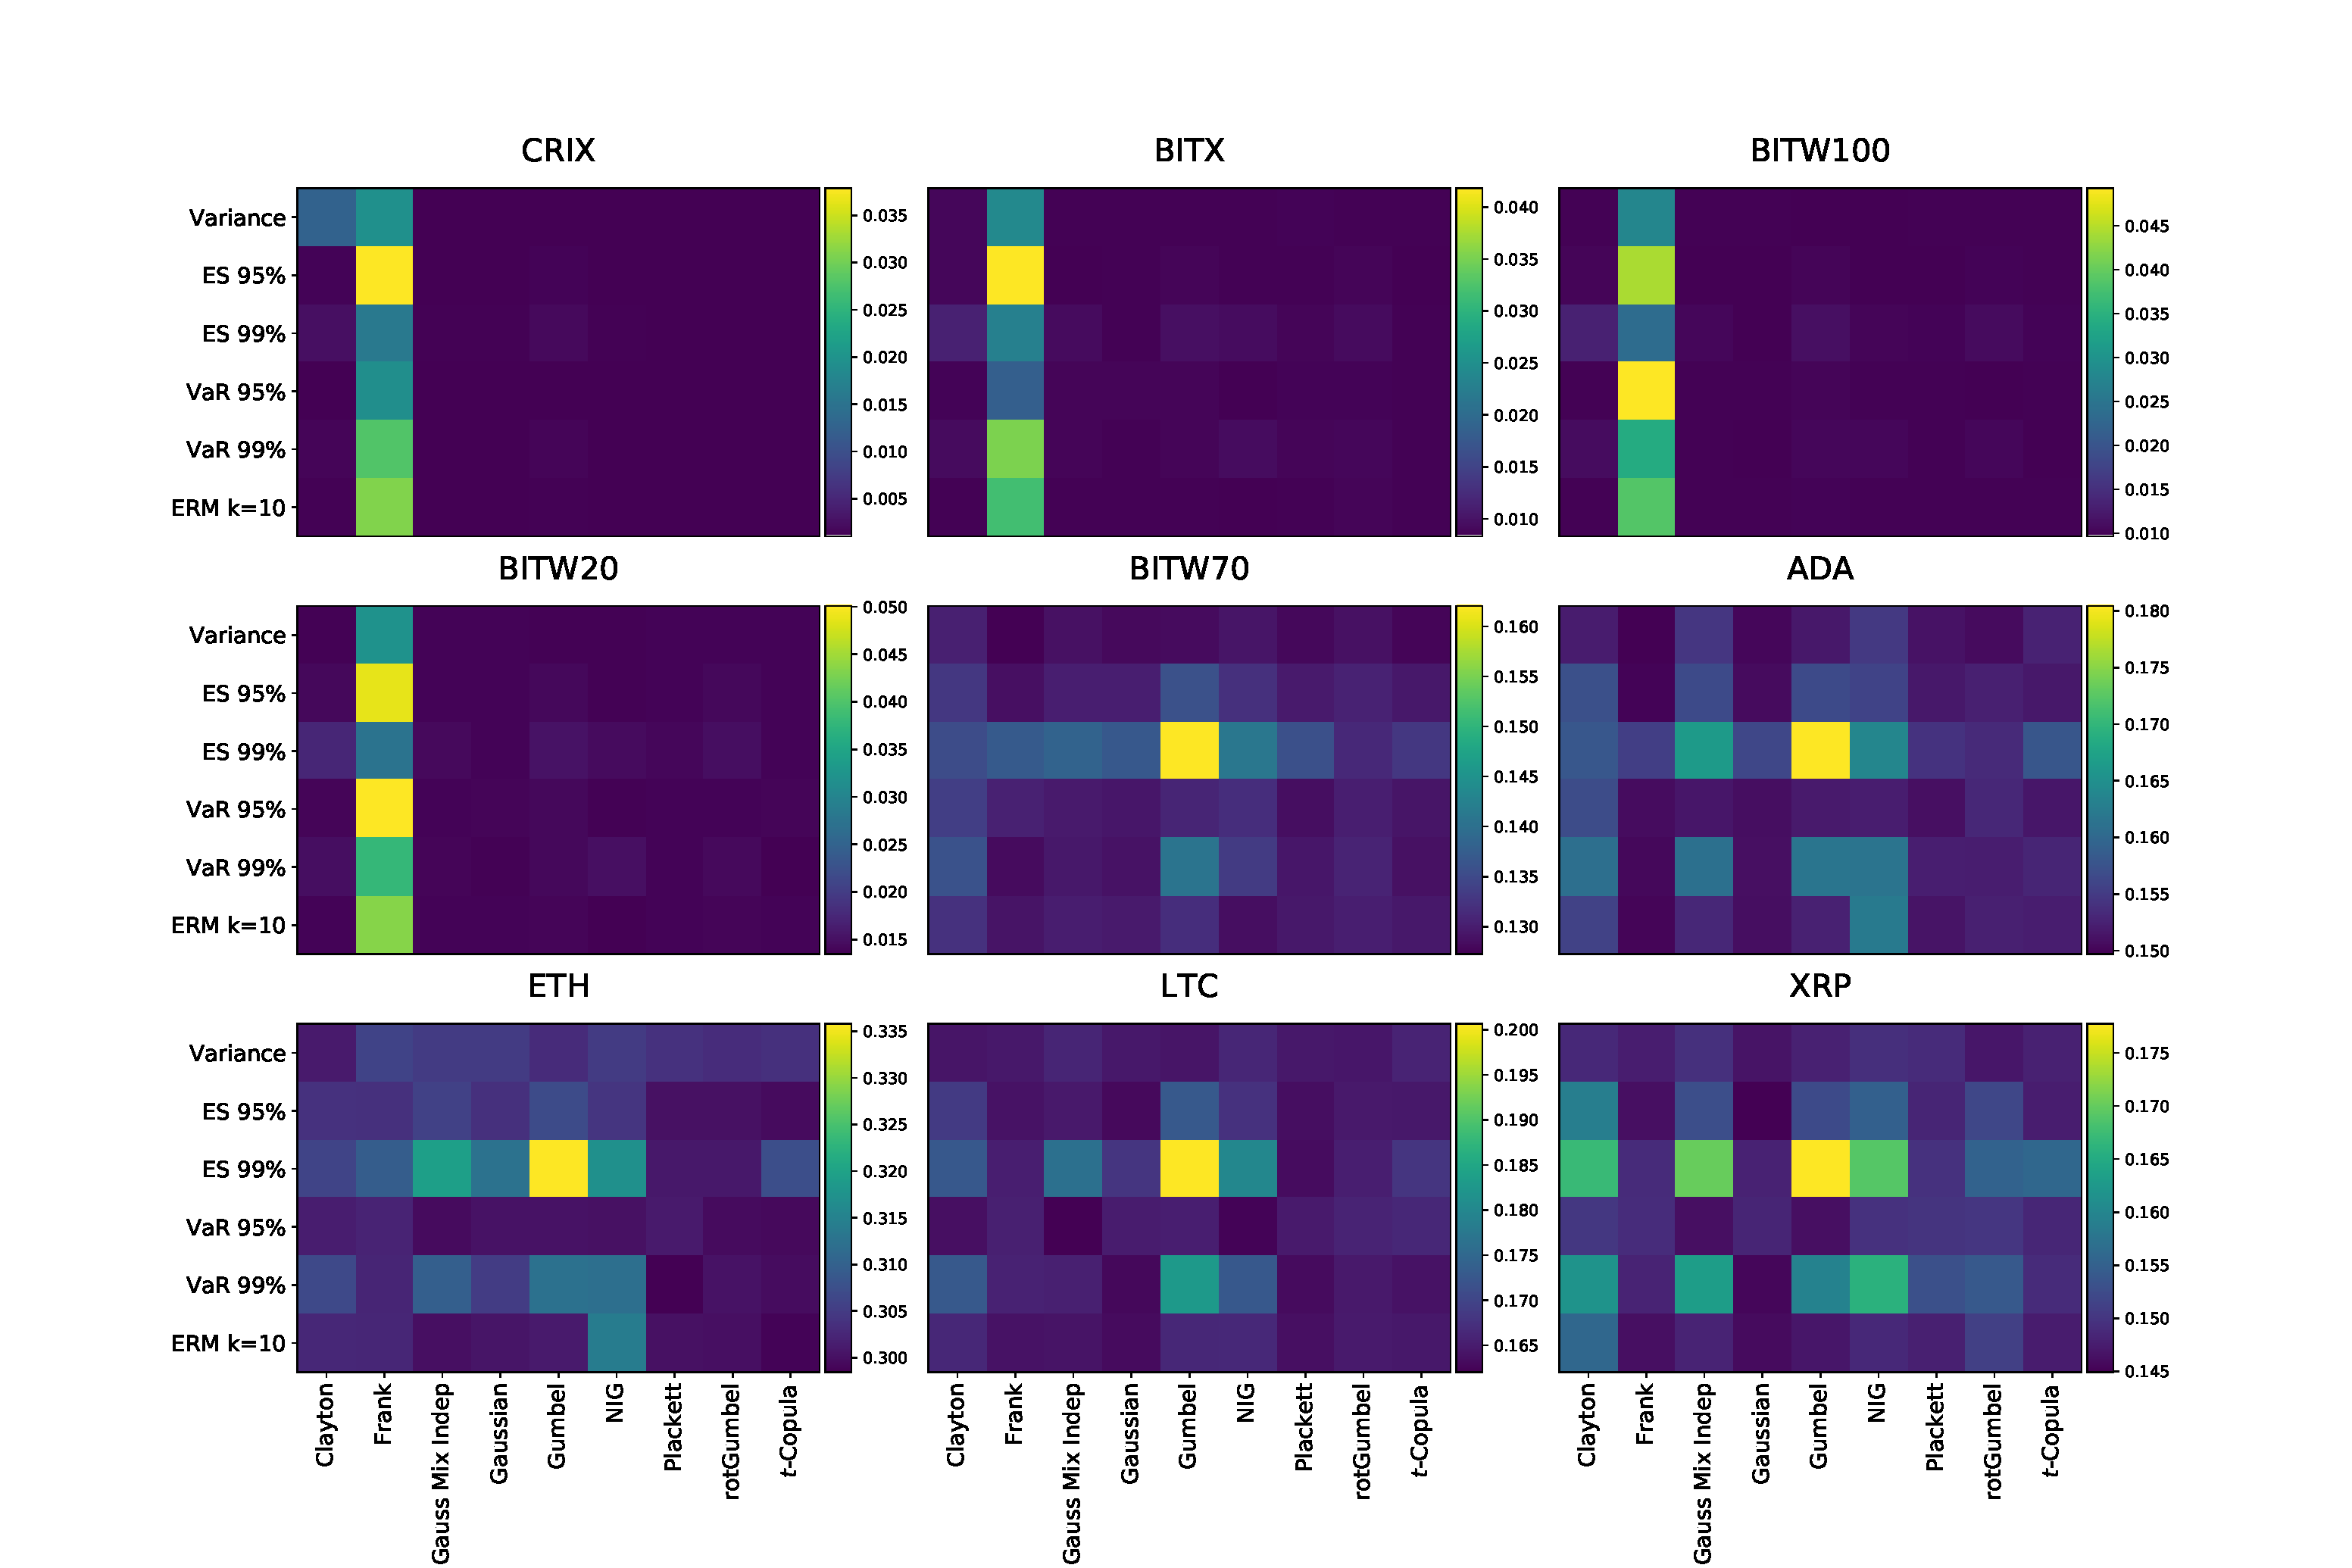
\includegraphics[width=\textwidth]{_pics/MSE_other.pdf}
  \caption{Mean square errors of portfolios constructed with different copula and risk minimization objectives.
  \href{http://www.quantlet.com/}{\includegraphics[height=\baselineskip]{_pics/qletlogo_tr.png}} }
\label{fig:MSE_other}
\end{figure}

\begin{figure}[th]
    \centering
    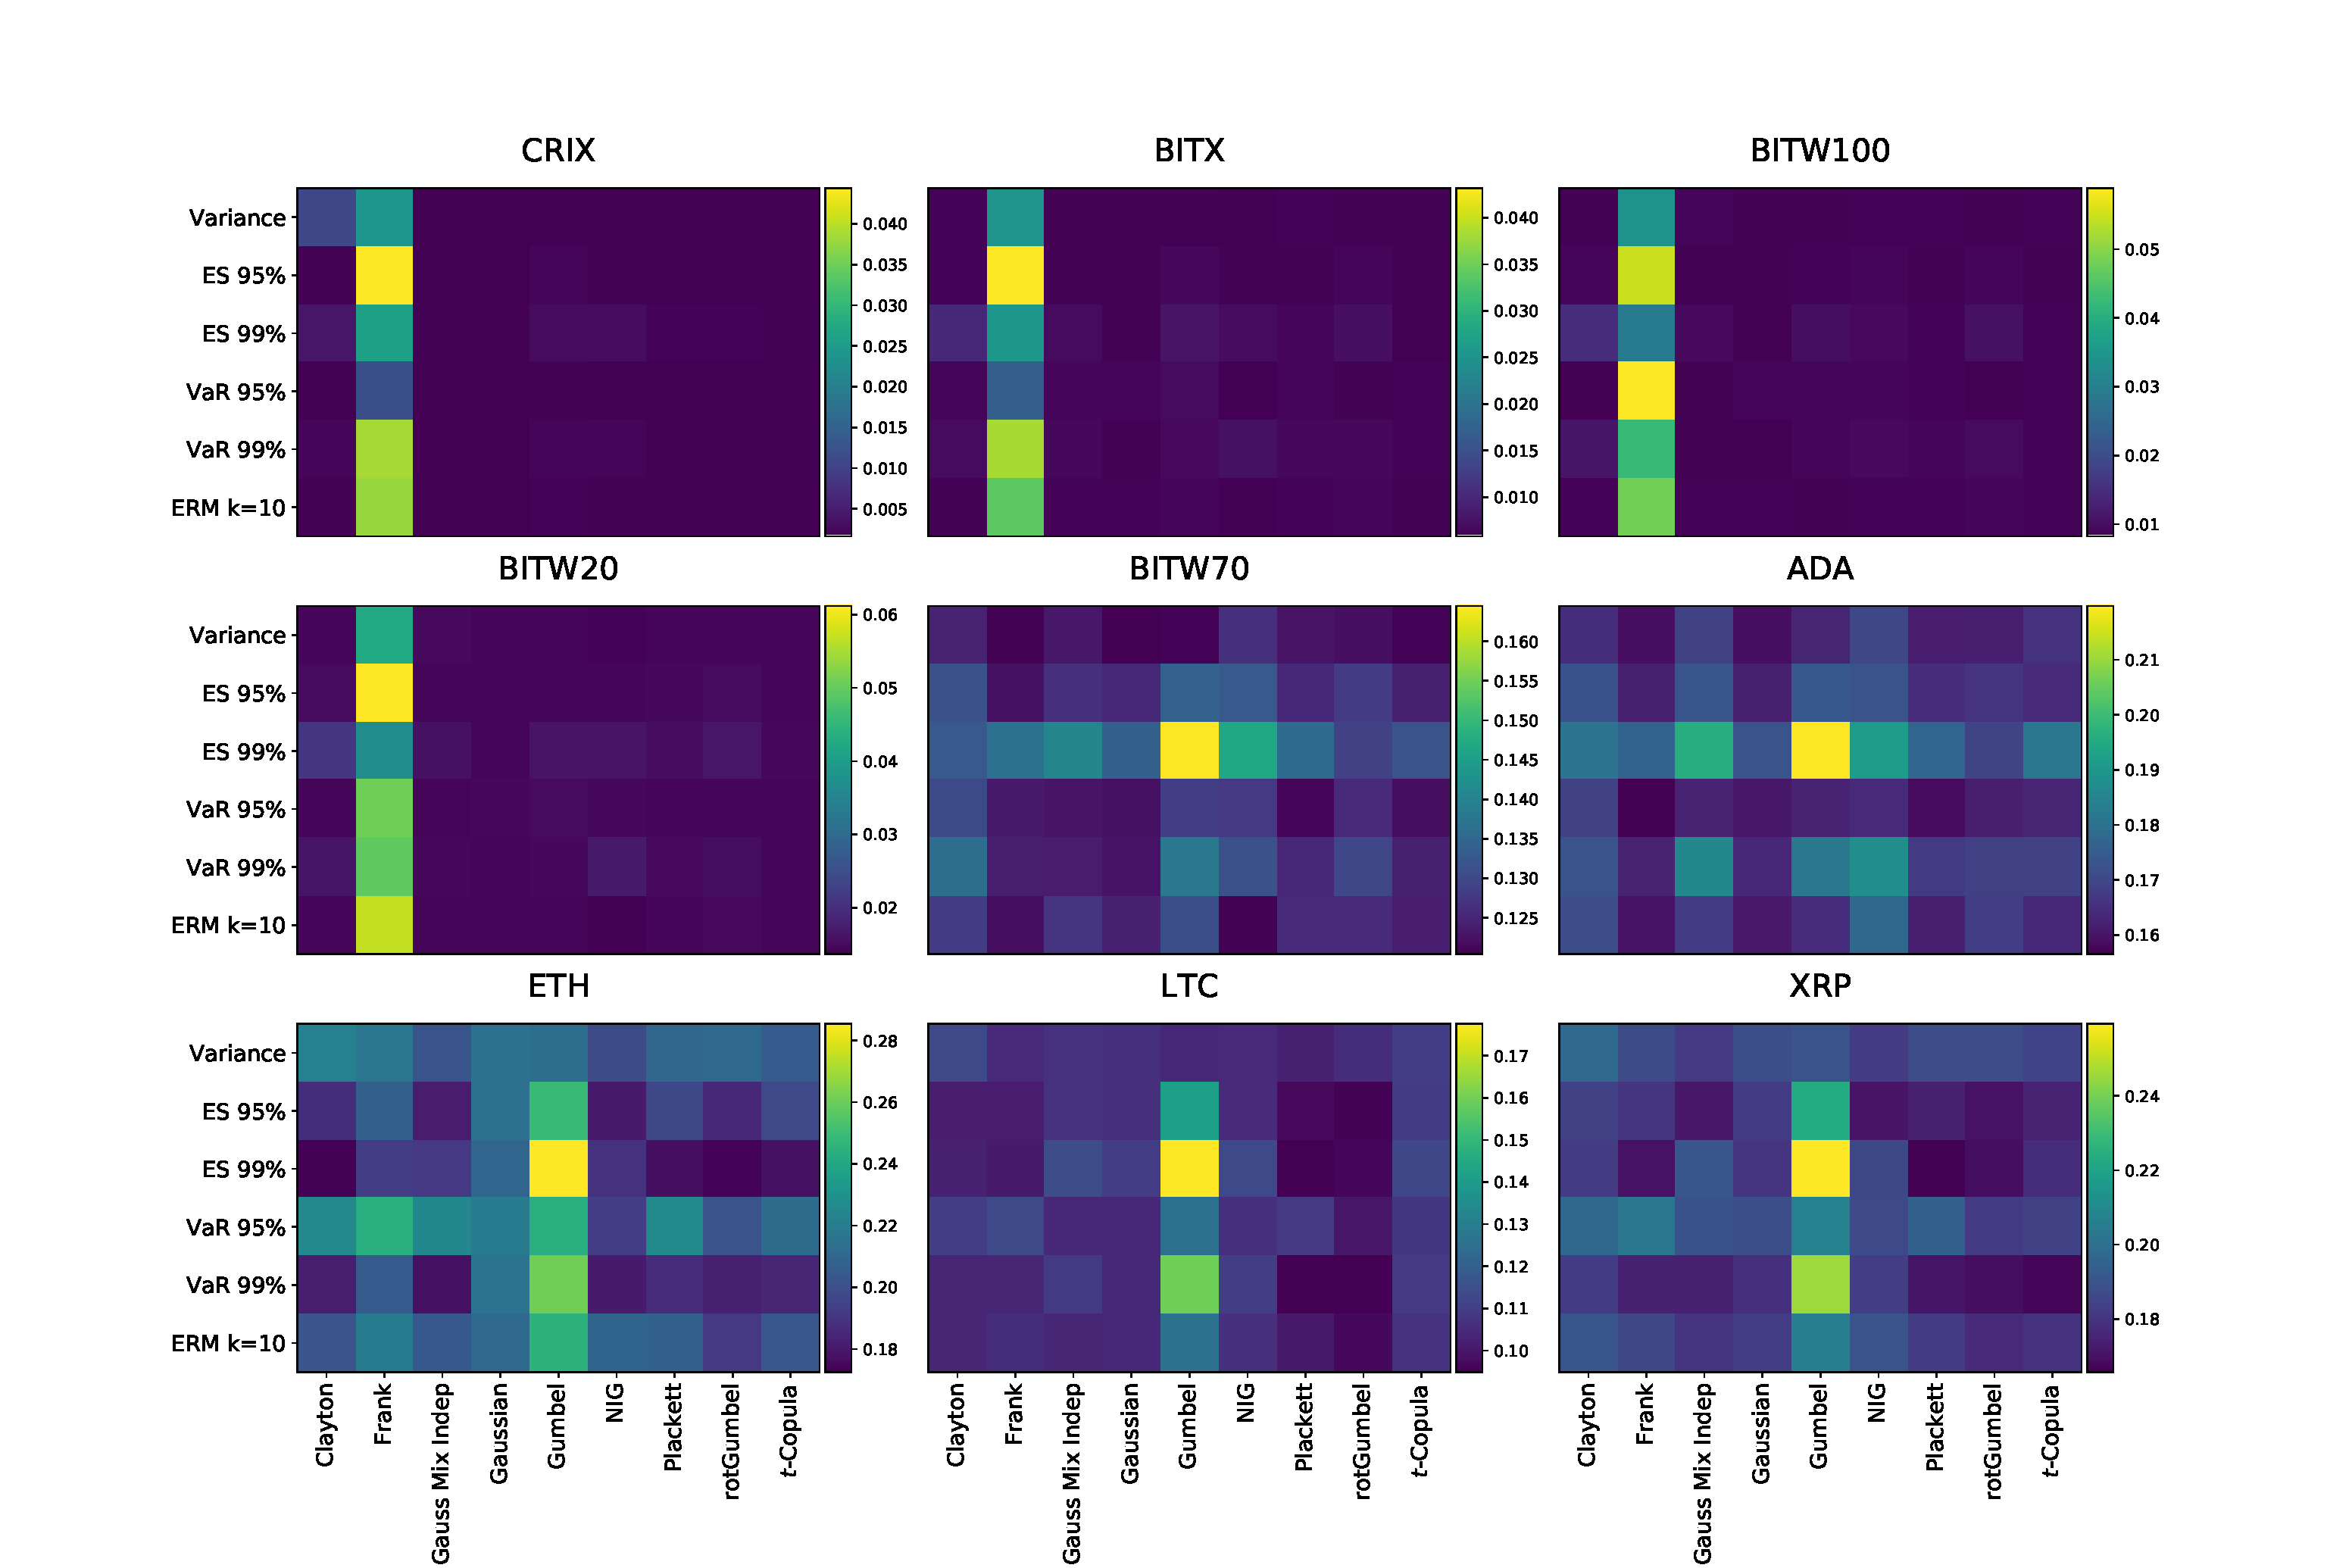
\includegraphics[width=\textwidth]{_pics/semiLowerVariance_other.pdf}
  \caption{Lower semivariance of portfolios constructed with different copula and risk minimization objectives.
  \href{http://www.quantlet.com/}{\includegraphics[height=\baselineskip]{_pics/qletlogo_tr.png}} }
\label{fig:SLV_other}
\end{figure}

\textcolor{darkblue}{As presented in Fig 3 and 4, either individual cryptos or indice, their cumulative returns dropped in Mar 2020. it's due to the result of COVID19. we can explain this for these two plots.}\\
\textcolor{darkblue}{Here i think it should insert a paragraph to interpret how you enter the copulae, otherwise it's weird that comes to Fig 5 and 6.}\\

Figure \ref{fig:MSE_BTC} and \ref{fig:SLV_BTC} are the mean square error and lower semivariance of BTC-BTCF, we can see the Frank copula is the worst performing copula:
the resulting hedged portfolio returns is far away from a perfect hedge.
In figure \ref{fig:MSE_other} and \ref{fig:SLV_other}, the phenomena of Frank copula being inferior to its counterparts can be observed from the results of the CRIX, BITX, BITW100, and BITW20-BTCF portfolios.
Interestingly, the spot in those portfolios usually have a strong dependency to the BTCF.
In contrast, the inferiority of the Frank copula is less prominent in the BITW70, ADA, ETH, LTC and XRP-BTCF portfolios.
We suspect that the Frank copula is not a choice to model assets with strong dependency. \textcolor{darkblue}{Frank copula is not appropriate for data that exhibit asymmetric and heavy tails.}  \medskip

We can also observe from figure \ref{fig:MSE_other} and \ref{fig:SLV_other} that Gumbel copula is not performing as good as other copula in the ETH, LTC, and XRP-BTCF portfolios.
The reason is the Gumbel copula has only the upper tail dependence, while the ETH, LTC, and XRP exhibit lower tail dependency with BTCF.
We will discuss this in the following section. \medskip

\subsection{Copula Selection Results}\label{sec: copula results}
\textcolor{darkblue}{Interpret the steps of copula selection.} \\
Next, we inspect the copula selection result.\textcolor{darkblue}{(I delete "in this section"...)}
Although the copula selection is only an intermediate step to obtain the OHRs,
the result of this step can help us better understand the dependence feature between BTCF and the assets we study in this work and give us
valuable information to model the assets in the future.
Decisions of the AIC procedure are summarised in table \ref{tab:copulasection}. \medskip

Overall, $t$-copula, rotated Gumbel (rotGumbel), and the NIG factor copula are the most frequently chosen copulae by the AIC procedure. \medskip

The $t$-copula is frequently chosen by AIC to model the dependency between the BTC and BTC involved indices, CRIX, BITX, BITW100, and the BTC future.
BTC and BTC involved indices exhibit strong tail dependence (both upper and lower tail) with BTCF.
We could interpret tail dependence much more of a tendency for one asset to be extreme when another is extreme and vice versa \citep{McNeil2015}.
In fact, the $t$ copula has been suggested in various empirical studies to model financial data, such as \cite{zeevi2002beyond} and \cite{breymann2003dependence}.
Those studies suggest $t$-copula is a better model over the Gaussian copula which financial data often seem to exhibit tail dependence. \textcolor{darkblue}{(because the thick and left skew properties of financial data tail distribution are documented. ))} \medskip

On the other hand, the radially symmetric feature makes the $t$-copula not a good choice to model the other hedging pairs.
\cite{demarta2005t} describe the symmetry feature "strong", because if $(U_1, ..., U_d)$ is a vector distributed in $t$-copula,
then $(U_1, ..., U_d) \overset{\mathcal{L}}= (1-U_1, ..., 1-U_d)$.
This symmetry can be justified in the dependence structure between a futures and its underlying by the theory of futures pricing,
which suggests the price of a futures is a function of the underlying price \citep{hull2003options}.
However, there is no such relationship between a futures and an asset which is not the underlying, and so the radial symmetry becomes a drawback to model other hedging pairs e.g. ETH and BITX70.
Another drawback of the $t$-copula is the lack of flexibility to model off-diagonal region since Rho and nu jointly control the density of the off-diagonal region.
%The off-diagonal region (HF paper breymann2003dependence)
This is why sometimes the Gaussian Mix Independence (GMI) better model the dependence.  \medskip

Among the three popular copulae, rotGumbel copula shows its ability to model the dependency between ETH and BTCF,
94 out of 112 training sets are best fitted with the rotated Gumbel.
rotGumbel also performs well when modelling dependency between XRP, BITW20, BITW70, and the BTCF.
In particular, the whole time series of the two indices, BITW20 and BITW70, are best fitted solely with the rotated Gumbel copula.
The frequently chosen rotated Gumbel indicates the styled fact of financial data: prices tends to drop together.  \medskip

In fact, Clayton's AIC in many of the training sets is the second lowest, just higher than that of rotated Gumbel.
This is because the Clayton copula has the same ability to model the lower quantile dependence.
However, Clayton's radial like feature does not match the behaviour of the financial data. \medskip

It is worth to mention that although the NIG factor copula is penalised heavily due to its three parameters setup, it is frequently chosen to be the best copula to model the dependency between individual cryptos and the BTC future.
An extreme case would be ADA, only NIG factor is chosen in our dataset.
Another dependency structure being best described by the NIG factor copula is the pair of LTC-BTCF.
64 out of 112 training sets are best fitted by the NIG factor copula.
Indices like BITX and CRIX are sometimes best fitted with the NIG factor copula as well, accounting for modelling 12 and 27 training sets respectively.
The popularity of the NIG factor reflects the ability of the copula to model very complex dependency structure.
NIG factor copula is able to model the tail, radial asymmetry, and off diagonal behaviour.  \medskip %(ADA samples and fitted NIG samples)

Frank copula is generally not a good choice to model financial data just like what \cite{barbi2014copula} has reported.
Plackett is known for its dependence parameter can be written as the cross-product ratio \citep{joe1997multivariate}.
However, this feature does not bring the Plackett Copula advantage over other copulae to model the dependence structure between cryptos and BTCF. \medskip

\begin{table}[t!]
 \ra{1.1}
    {\begin{tabularx}{\textwidth}{lYYYYY} \toprule
         Copula/Asset & $t$ & Plackett & GMI & rotGumbel & NIG \\ \midrule
     \multicolumn{6}{l}{Individual Cryptos}                                                                                 \\
        \ \ \ BTC          & 73         & 4                 & 2                        & 1                  & 31                  \\
        \ \ \ ETH          & 3          & 6                 & 8                        & 94                 & 1                   \\
        \ \ \ ADA          & 0          & 0                 & 0                        & 0                  & 112                 \\
        \ \ \ LTC          & 13         & 0                 & 3                        & 32                 & 64                  \\
        \ \ \ XRP          & 0          & 31                & 3                        & 78                 & 0                   \\
   \multicolumn{6}{l}{Crypto Indices with BTC Constituent}                                                                  \\
        \ \ \ BITX         & 39         & 0                 & 14                       & 16                 & 12                  \\
        \ \ \ CRIX         & 47         & 0                 & 11                       & 3                  & 27                  \\
        \ \ \ BITW100      & 42         & 0                 & 8                        & 29                 & 2                   \\
    \multicolumn{6}{l}{Crypto Indices without BTC Constituent}                                                              \\
        \ \ \ BITW20       & 0          & 0                 & 0                        & 78                 & 3                   \\
        \ \ \ BITW70       & 0          & 0                 & 0                        & 80                 & 1                   \\
    \bottomrule
    \end{tabularx}
        \caption{Copula Selection Results. }









% \ra{1.1}
    {\begin{tabularx}{\textwidth}{lrrrrrrrr} \toprule
         {} &    Mean \% &     Std \% &      Skew &       Kurt &         MD &     MD date \\
\midrule
     \multicolumn{8}{l}{Hedging Instrument}
\textbackslash  \textbackslash  \textbackslash  BTCF &    0.39 &   4.63 & -0.51 &   4.42 & -26.99 &  2020-03-12 \\
     \multicolumn{8}{l}{Individual Cryptos}                                                                                 \\
BTC        &    0.39 &   4.40 & -0.59 &   4.66 & -26.00 &  2020-03-12 \\
ETH        &    0.68 &   6.01 & -0.26 &   5.26 & -32.01 &  2020-03-12 \\
ADA        &    0.95 &   6.70 &  0.17 &   2.31 & -26.85 &  2020-03-12 \\
LTC        &    0.32 &   6.48 & -0.99 &   5.30 & -37.59 &  2021-05-19 \\
XRP        &    0.30 &   7.98 &  0.55 &  12.49 & -52.77 &  2020-12-23 \\
   \multicolumn{8}{l}{Crypto Indices with BTC Constituent}                                                                  \\
BITX       &    0.21 &   4.74 & -0.55 &   4.04 & -27.02 &  2020-03-12 \\
CRIX       &    0.22 &   4.70 & -0.49 &   4.16 & -27.14 &  2020-03-12 \\
BITW100    &    0.22 &   4.76 & -0.63 &   4.03 & -27.27 &  2020-03-12 \\
    \multicolumn{8}{l}{Crypto Indices without BTC Constituent}                                                              \\
BITW20     &    0.18 &   5.50 & -0.90 &   3.72 & -31.01 &  2020-03-12 \\
BITW70     &    0.17 &   5.85 & -0.96 &   4.11 & -32.35 &  2021-05-19 \\
    \bottomrule
    \end{tabularx}
        \caption{Copula Selection Results. }
    \label{tab:copulasection}}
\end{table}

\subsection{Hedged portfolios with the copula selection step}\label{subsec:HP2}
We presents the TBC

\begin{table}[!] \centering \resizebox{\textwidth}{!}{%
\begin{tabular}{lrrrrrrr} \toprule
         {} &    Mean \% &     Std \% &      Skew &       Kurt &         MD \% &     MD date & ERM k=10 \\
\midrule
     \multicolumn{7}{l}{Individual Cryptos}                                                                                 \\
\ \ \ BTC     &  0.0223 &  0.3221 & -1.0008 &   3.4153 &  -1.5242 &  2020-11-30 &    0.0057 \\
\ \ \ ETH     &  0.3117 &  3.8679 &  1.0345 &   7.5751 & -18.8729 &  2021-05-19 &    0.0491 \\
\ \ \ ADA     &  0.5722 &  5.3590 &  1.4203 &   4.6970 & -14.3885 &  2021-01-08 &    0.0700 \\
\ \ \ LTC     & -0.0512 &  3.8812 & -0.2929 &   7.7022 & -28.0879 &  2021-05-19 &    0.0616 \\
\ \ \ XRP     &  0.0155 &  7.1579 &  1.1244 &  19.8583 & -52.5689 &  2020-12-23 &    0.0787 \\
   \multicolumn{7}{l}{Crypto Indices with BTC Constituent}                                                                  \\
\ \ \ BITX    &  0.0590 &  1.0078 & -0.4427 &  13.0839 &  -7.8581 &  2021-05-19 &    0.0127 \\
\ \ \ CRIX    &  0.0840 &  0.9087 &  0.0488 &  14.5501 &  -7.0530 &  2021-05-19 &    0.0100 \\
\ \ \ BITW100 &  0.0853 &  1.2032 & -1.6522 &  20.5562 & -11.1846 &  2021-05-19 &    0.0153 \\
    \multicolumn{7}{l}{Crypto Indices without BTC Constituent}                                                              \\
\ \ \ BITW20  &  0.2564 &  3.6009 & -0.3446 &   4.2152 & -21.5920 &  2021-05-19 &    0.0503 \\
\ \ \ BITW70  &  0.2818 &  3.9074 & -0.6952 &   4.8745 & -24.5250 &  2021-05-19 &    0.0557 \\
\bottomrule
\end{tabular}}
\caption{Summary statistics of out-of-sample daily returns of hedged portfolios that minimize ERM $k=10$.}
\label{tab:ERM_rh}

\end{table}

\begin{table}[!] \centering \resizebox{\textwidth}{!}{%
\begin{tabular}{lrrrrrrr} \toprule
         {} &    Mean \% &     Std \% &      Skew &       Kurt &         MD \% &     MD date & ES 5\% \\
\midrule
     \multicolumn{7}{l}{Individual Cryptos}                                                                                 \\
\ \ \ BTC     &  0.0204 &  0.3234 & -1.0150 &   3.4423 &  -1.5629 &  2020-11-30 &  0.0101 \\
\ \ \ ETH     &  0.3082 &  3.8890 &  1.0119 &   7.4077 & -18.7819 &  2021-05-19 &  0.0782 \\
\ \ \ ADA     &  0.5525 &  5.2673 &  1.2557 &   4.2423 & -14.9647 &  2021-05-19 &  0.0984 \\
\ \ \ LTC     & -0.0808 &  3.9829 & -0.4957 &   7.2302 & -28.4608 &  2021-05-19 &  0.0962 \\
\ \ \ XRP     &  0.0176 &  7.1533 &  1.1411 &  19.9176 & -52.5698 &  2020-12-23 &  0.1354 \\
   \multicolumn{7}{l}{Crypto Indices with BTC Constituent}                                                                  \\
\ \ \ BITX    &  0.0591 &  1.0065 & -0.3453 &  12.1335 &  -7.6211 &  2021-05-19 &  0.0215 \\
\ \ \ CRIX    &  0.0777 &  0.9207 &  0.0164 &  13.5608 &  -6.9894 &  2021-05-19 &  0.0173 \\
\ \ \ BITW100 &  0.0848 &  1.2125 & -1.6397 &  19.7472 & -11.1357 &  2021-05-19 &  0.0274 \\
    \multicolumn{7}{l}{Crypto Indices without BTC Constituent}                                                              \\
\ \ \ BITW20  &  0.2608 &  3.6115 & -0.3555 &   4.2016 & -21.5430 &  2021-05-19 &  0.0804 \\
\ \ \ BITW70  &  0.2785 &  3.9157 & -0.6949 &   4.8047 & -24.3474 &  2021-05-19 &  0.0908 \\
\bottomrule
\end{tabular}}
\caption{Summary statistics of out-of-sample daily returns of hedged portfolios that minimize ES 5\%.}
\label{tab:ES5_rh}

\end{table}
\begin{table}[th] \centering \resizebox{\textwidth}{!}{%
\begin{tabular}{lrrrrrrr} \toprule
         {} &    Mean \% &     Std \% &      Skew &       Kurt &         MD \% &     MD date & ES 1\% \\
\midrule
     \multicolumn{7}{l}{Individual Cryptos}                                                                                 \\
\ \ \ BTC     &  0.0148 &  0.3476 & -0.8354 &   3.3054 &  -1.6225 &  2020-11-30 &  0.0234 \\
\ \ \ ETH     &  0.3080 &  3.8954 &  0.9840 &   7.4947 & -18.7625 &  2021-05-19 &  0.1299 \\
\ \ \ ADA     &  0.5016 &  5.4040 &  1.1008 &   3.9607 & -15.4481 &  2021-05-19 &  0.1463 \\
\ \ \ LTC     & -0.1029 &  4.1581 & -0.7757 &   7.4375 & -29.1727 &  2021-05-19 &  0.1647 \\
\ \ \ XRP     & -0.0200 &  7.2887 &  1.1121 &  18.8732 & -52.5700 &  2020-12-23 &  0.2516 \\
   \multicolumn{7}{l}{Crypto Indices with BTC Constituent}                                                                  \\
\ \ \ BITX    &  0.0598 &  1.0312 & -0.4410 &  11.5863 &  -7.7424 &  2021-05-19 &  0.0411 \\
\ \ \ CRIX    &  0.0835 &  0.9461 & -0.0361 &  12.4047 &  -7.0203 &  2021-05-19 &  0.0350 \\
\ \ \ BITW100 &  0.0781 &  1.2640 & -1.9645 &  21.8836 & -11.9263 &  2021-05-19 &  0.0593 \\
    \multicolumn{7}{l}{Crypto Indices without BTC Constituent}                                                              \\
\ \ \ BITW20  &  0.2538 &  3.6323 & -0.4086 &   4.4462 & -21.9866 &  2021-05-19 &  0.1282 \\
\ \ \ BITW70  &  0.2660 &  3.9320 & -0.7598 &   5.0050 & -24.4764 &  2021-05-19 &  0.1535 \\
\bottomrule
\end{tabular}
}
\caption{Summary statistics of out-of-sample daily returns of hedged portfolios that minimize ES 1\%.}
\label{tab:ES1_rh}

\end{table}
\begin{table}[th] \centering \resizebox{\textwidth}{!}{%
\begin{tabular}{lrrrrrrr} \toprule
         {} &    Mean \% &     Std \% &      Skew &       Kurt &         MD \% &     MD date & VaR 5\% \\
\midrule
     \multicolumn{7}{l}{Individual Cryptos}                                                                                 \\
\ \ \ BTC     &  0.0253 &  0.3294 & -0.9725 &   3.4373 &  -1.5347 &  2020-11-30 &  0.0063 \\
\ \ \ ETH     &  0.3084 &  3.8944 &  1.0243 &   7.4297 & -19.1750 &  2021-05-19 &  0.0514 \\
\ \ \ ADA     &  0.5726 &  5.2204 &  1.2981 &   4.2544 & -14.6974 &  2021-05-19 &  0.0769 \\
\ \ \ LTC     & -0.0742 &  3.9145 & -0.3836 &   7.5384 & -28.3672 &  2021-05-19 &  0.0622 \\
\ \ \ XRP     &  0.0208 &  7.1520 &  1.1269 &  19.8930 & -52.5667 &  2020-12-23 &  0.0683 \\
   \multicolumn{7}{l}{Crypto Indices with BTC Constituent}                                                                  \\
\ \ \ BITX    &  0.0562 &  0.9930 & -0.3117 &  12.4780 &  -7.5639 &  2021-05-19 &  0.0128 \\
\ \ \ CRIX    &  0.0863 &  0.9151 &  0.0718 &  13.7915 &  -6.9744 &  2021-05-19 &  0.0092 \\
\ \ \ BITW100 &  0.0846 &  1.1980 & -1.6592 &  21.3725 & -11.2582 &  2021-05-19 &  0.0164 \\
    \multicolumn{7}{l}{Crypto Indices without BTC Constituent}                                                              \\
\ \ \ BITW20  &  0.2728 &  3.5940 & -0.3721 &   4.4896 & -22.0733 &  2021-05-19 &  0.0546 \\
\ \ \ BITW70  &  0.2847 &  3.9133 & -0.6580 &   4.7874 & -24.6513 &  2021-05-19 &  0.0626 \\
\bottomrule
\end{tabular}}
\caption{Summary Statistics of Hedged Portfolios that minimize VaR 5\%.}
\label{tab:VaR5_rh}

\end{table}
\begin{table}[th] \centering \resizebox{\textwidth}{!}{%
\begin{tabular}{lrrrrrrr} \toprule
         {} &    Mean \% &     Std \% &      Skew &       Kurt &         MD \% &     MD date & VaR 5\% \\
\midrule
     \multicolumn{7}{l}{Individual Cryptos}                                                                                 \\
\ \ \ BTC     &  0.0176 &  0.3270 & -1.0405 &   3.3742 &  -1.5689 &  2020-11-30 &  0.0134 \\
\ \ \ ETH     &  0.2977 &  3.9132 &  0.9547 &   7.2414 & -18.6061 &  2021-05-19 &  0.1026 \\
\ \ \ ADA     &  0.5562 &  5.3466 &  1.1362 &   3.9334 & -15.4795 &  2021-05-19 &  0.1106 \\
\ \ \ LTC     & -0.0852 &  4.1503 & -0.7234 &   7.3208 & -29.0915 &  2021-05-19 &  0.1030 \\
\ \ \ XRP     &  0.0352 &  7.1658 &  1.1582 &  19.8506 & -52.5727 &  2020-12-23 &  0.1387 \\
   \multicolumn{7}{l}{Crypto Indices with BTC Constituent}                                                                  \\
\ \ \ BITX    &  0.0593 &  1.0178 & -0.5331 &  13.3100 &  -8.0299 &  2021-05-19 &  0.0247 \\
\ \ \ CRIX    &  0.0738 &  0.9695 & -0.4729 &  13.6500 &  -7.0185 &  2021-05-19 &  0.0245 \\
\ \ \ BITW100 &  0.0823 &  1.2338 & -1.9365 &  23.1938 & -11.8752 &  2021-05-19 &  0.0347 \\
    \multicolumn{7}{l}{Crypto Indices without BTC Constituent}                                                              \\
\ \ \ BITW20  &  0.2499 &  3.6210 & -0.3866 &   4.3396 & -21.6634 &  2021-05-19 &  0.0988 \\
\ \ \ BITW70  &  0.2788 &  3.9257 & -0.7635 &   5.1288 & -24.5294 &  2021-05-19 &  0.1147 \\
\bottomrule
\end{tabular}}
\caption{Summary statistics of out-of-sample daily returns of hedged portfolios that minimize VaR 1\%.}
\label{tab:VaR1_rh}

\end{table}
\include{_tables/var1_rh}

\subsection{Hedging Effectiveness Results}\label{sec: HE results}
In this section, we analyse the out-of-sample hedging effectiveness (HE) of BTCF as hedging.
HE is defined as $$\text{HE} = 1-\frac{\rho_h}{\rho_s},$$
a measure of the percentage reduction of portfolio risk attribute, in our case the spot $\rho_s$,
to hedged portfolio risk attribute $\rho_h$.
A higher HE indicates a higher hedging effectiveness and larger risk reduction. \medskip

The HE above is a generalisation of Ederington measure of hedging performance, where we,
in addition to variance, include other risk measures: Expected Shortfall 5\% and 1\% (ES5 and ES1), Value-at-Risk 5\% and 1\% (VaR5 and VaR1), and ERM.
In particular, ES5 is recommended by the Basel Committee on Banking Supervision (BCBS) to replace VaR as a quantitative risk metrics system.
The proposed reform aimed at enhancing the risk metric system's ability to capture tail risk. \medskip
%Discussions of the issue can be found in literatures.
%
We obtain a time series of out-of-sample $r^h$ of each hedging pair and each risk reduction objective by concatenating the out-of-sample results.
Then, we apply stationary block bootstrapping (SB) to the time series introduced by \cite{Politis1994} in our analysis in order to preserve the temporal structure of the data while sampling.
The SB procedure is as follow.
Assume a time series with $N$ observations $\{X_t\}_{t \in [1,N]}$ is a strong stationary, weakly dependence time series of interest,
we form blocks of samples $B = \{X_i, ..., X_{i+j-1}\}$.
Index $i$ is a random variable uniformly distributed over $[1,2,...,N]$ and $j$ is geometric distributed random variable with parameter .
The block index $i$ and block length $j$ are independent.
For any index $k$ which is greater than $N$, the sample $X_k$ is defined to be $X_{k(\mod N)}$.
For each block, we calculate the hedging effectiveness with different risk measures mentioned above.
We choose $p=0.005$, implying the expected block length is 200.
100 blocks are drawn for each risk minimising objective and spot. \medskip

From figure \ref{fig:HEboxplot}, we report, as expected, the BTC involving spots, the BTC, CRIX, BITX and BITW100, are well hedged by the BTCF.
Surprisingly, the performances are consistent across different risk reduction objectives and different HE evaluation.
The median HE to BTC generated by various risk reduction objectives is ranging from 89.45\% to 99.31\%, median HE to CRIX is ranging from 81.13\% to 95.22\%,
median HE to BITX is ranging from 79.06\% to 94.84\%, median HE to BITW100 Is ranging from 71.07\% to 92.98\%. \medskip

The HE of BTCF to other cryptos and indices are substantially lower than to the BTC involving spots, but the consistency the performances across different risk reduction objectives and HE evaluation remains.
The median HE to BITW20 generated by various risk reduction objectives is ranging from 24.67\% to 47.02\%, median HE to BITW70 is ranging from 23.61\% to 49.30\%,
median HE to ADA is ranging from 9.01\% to 29.30\%, median HE to ETH Is ranging from 30.07\% to 36.18\%, median HE to LTC Is ranging from 37.74\% to 51.30\%,
median HE to XRP Is ranging from 0.46\% to 30.89\%.
\begin{figure}[h]
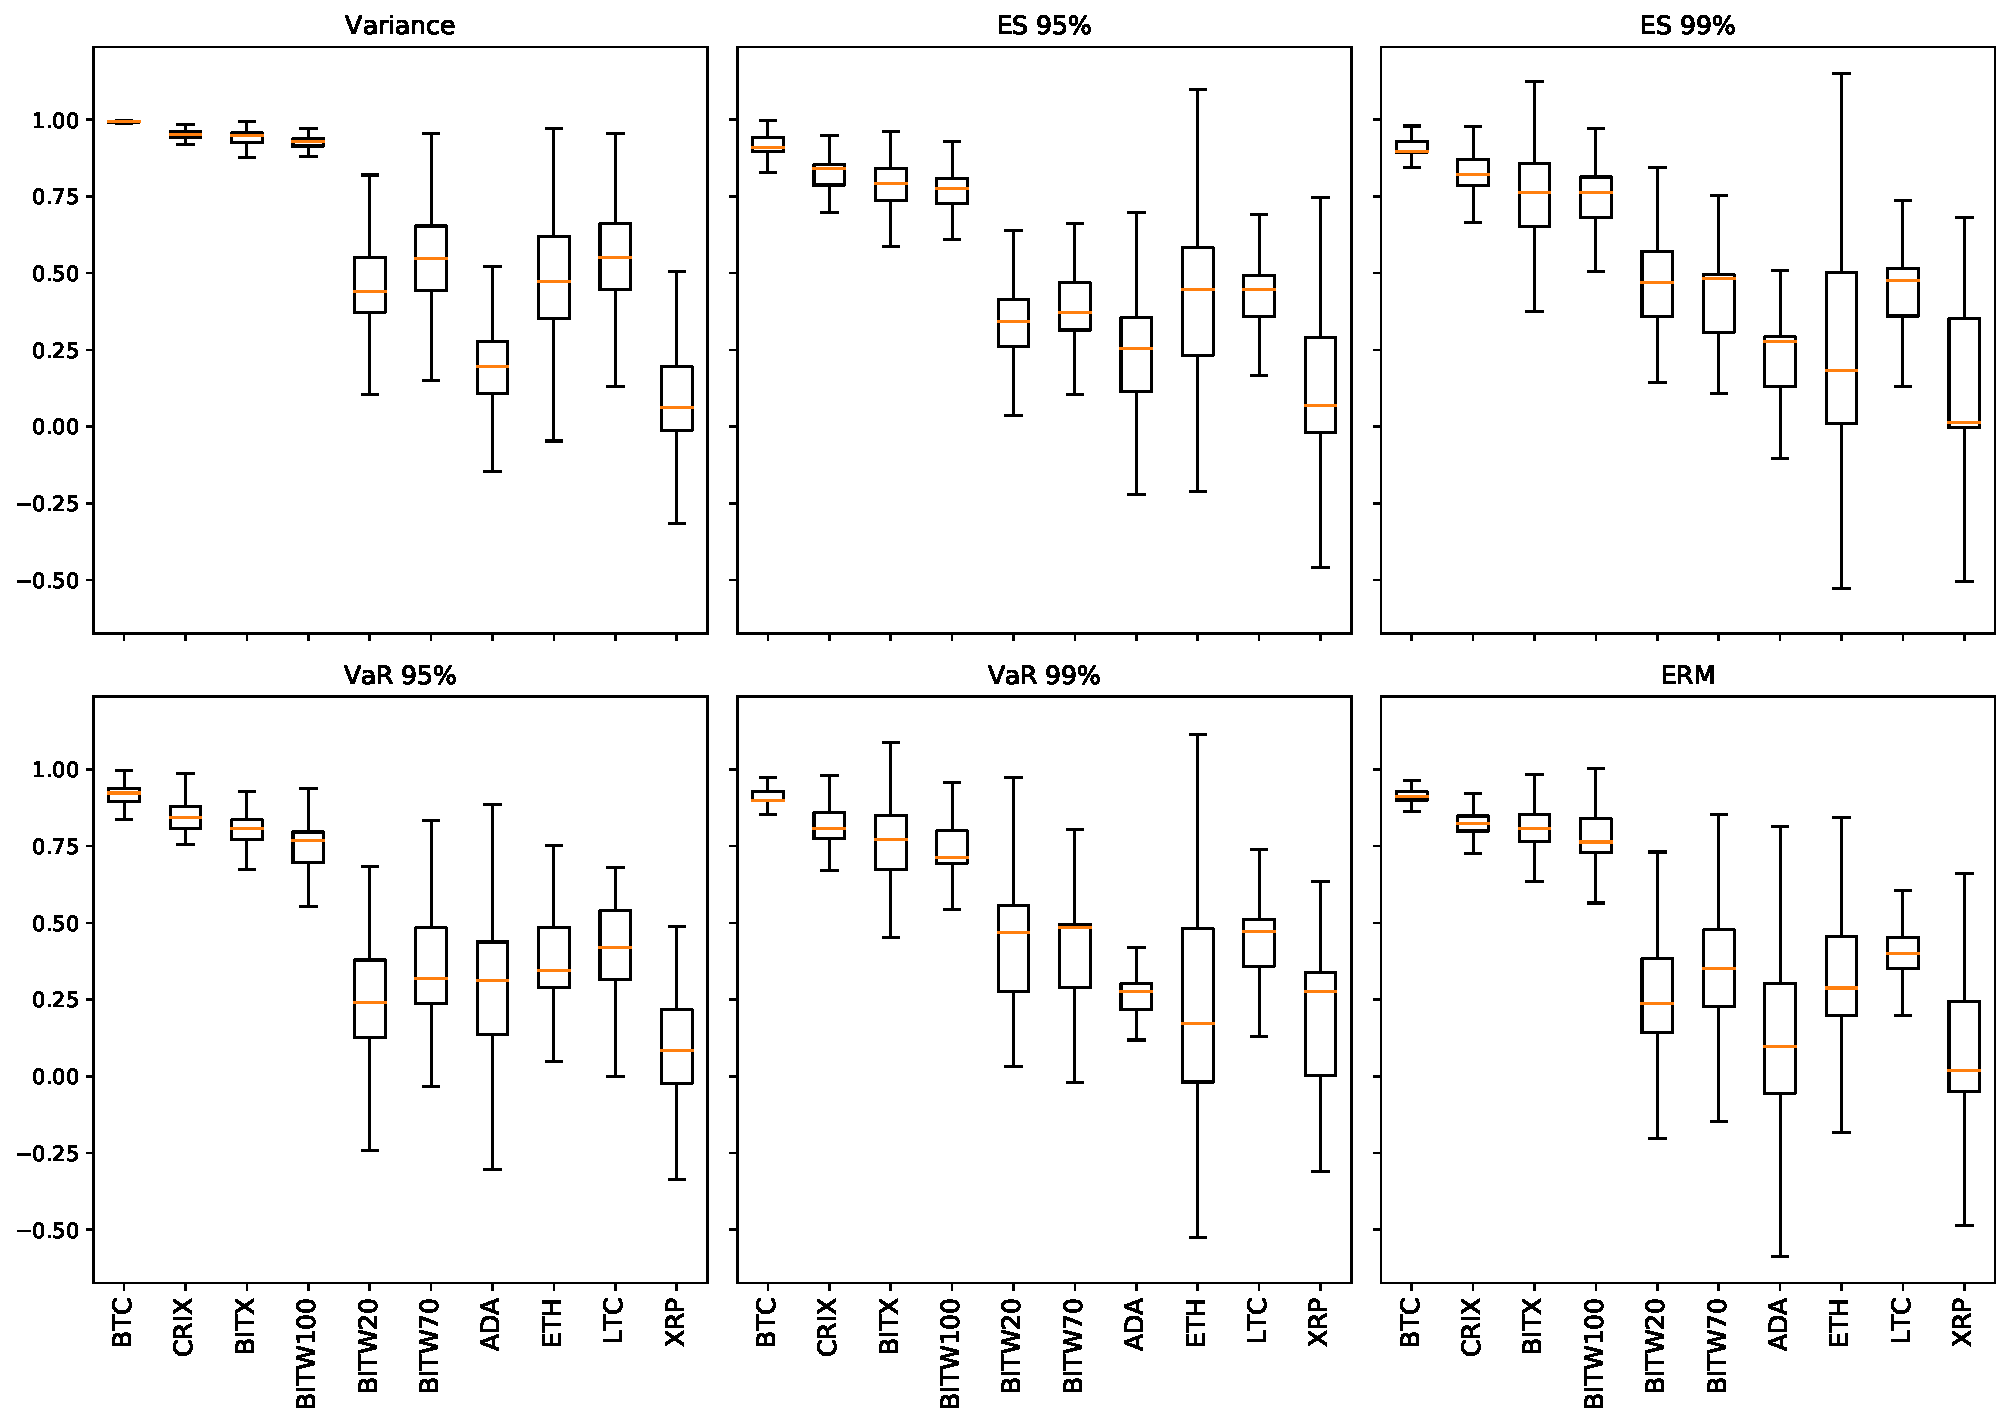
\includegraphics[width=\textwidth]{_pics/ES5_HE_boxplot.pdf}
  \caption{HE evaluated in the corresponding risk minimization objectives.
            The boxplots indicate the the median, upper quartile, lower quartile, minimium and maximum of the bootstrapped HE.
            The HE of BTC-involved spots are significantly higher than that of BTC-not-involved spots.
  \href{http://www.quantlet.com/}{\includegraphics[height=\baselineskip]{_pics/qletlogo_tr.png}} }
\label{fig:HEboxplot}
\end{figure}